\documentclass[12pt,journal,onecolumn]{IEEEtran}

%% ** Style Notice **
%% **Different IEEE style can be chosen by changing \documentclass[12pt,journal,onecolumn]{IEEEtran} to \documentclass[12pt,conference,onecolumn] and etc.
%% ** For detail info please visit IEEE_Original folder and check IEEEtran_HOWTO.pdf
%% ** One Column style with normal font of 12 pt is set, delete onecolumn in doucumentclass if you need double column
%% ** Style is mainly based on IEEEtrans template and if you want to change different line distance or font scale, check IEEEtran_HOWTO.pdf
%% ** Tested in Microsoft Visual Studio Code, with Latex-Workshop extension, texlive2018 environment installed. No guarantee on other platform (linux or mac) or other tex environment.

%% ** 这个不是天大毕业论文模板,应付普通大作业/结课报告用的
%% ** 此模板图,表,章节标题默认中文
%% ** 模板基于IEEEtran
%% ** 其实看着很奇怪,就凑合这样了
%% ** 其实只用封皮就可以了---溜走
%% ** github已有很多天大中文的毕业论文模板,要想用比较符合中文的报告模板可以直接拿来用了
%% ** 字号,行间距,缩进等修改请仍然参考IEEEtran_HOWTO.pdf
%% ** 模板没有对IEEEtran.cls修改(patchcmd很好用)
%% ** IEEE模板有很多样式,journal, conference等,可以更改第一行\documentclass参数来修改,参考IEEEtran_HOWTO.pdf(比如conference的页码就在底部)
%% ** 编辑环境为Windows+VSCode+Latex-Workshop extension+texlive2018,已知mac和linux中文显示会跟Windows不同,控制序列\songti不可用,不保证其他平台可用性....请参考ctex手册对照自己平台修改...

\usepackage[pdftex]{graphicx}
\DeclareGraphicsExtensions{.pdf,.jpeg,.png,.eps}
\usepackage{svg}
\usepackage{epstopdf}
\usepackage{cite}
\usepackage{amsmath}
\usepackage{algorithmic}
\usepackage{array}
\usepackage{amsfonts,amssymb}
\usepackage{textcomp}
\ifCLASSOPTIONcompsoc
 \usepackage[caption=false,font=normalsize,labelfont=sf,textfont=sf]{subfig}
\else
 \usepackage[caption=false,font=footnotesize]{subfig}
\fi
\usepackage{url}
\usepackage[hidelinks]{hyperref}

\usepackage[UTF8,scheme=chinese]{ctex} % Add support for Chinese characters.

% \usepackage[english]{babel} % Incase you have some special french or other characters in your bib and main tex. Comment out if you don't need. English Environment

\usepackage{caption} % Reduce the space after caption.
\captionsetup{font=scriptsize}
\setlength\belowcaptionskip{-8pt}

\usepackage[autostyle]{csquotes} %Resolve quotation mark  direction problems.
\MakeOuterQuote{"} % English Environment only

\usepackage{etoolbox} % Use patchcmd to control alignment of section title.

\hyphenation{semi-conduc-tor} % Avoid unwanted hyphenation.


\begin{document}

% this is the Cover
\begin{center}
  \quad
  
  \vspace{1cm}
  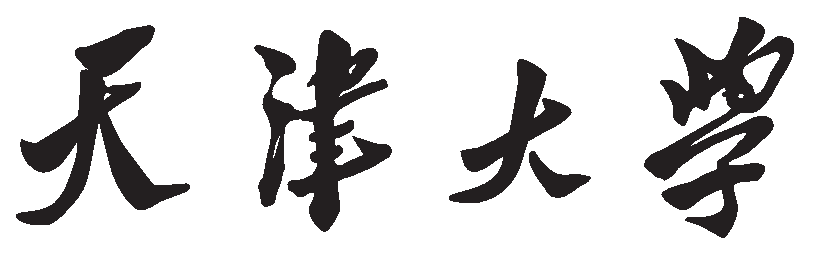
\includegraphics[width=7cm]{./logo/TDFonts.eps}
  \vspace{2cm}


  {
  \fontfamily{phv}
  \fontsize{24}{30}
  \selectfont \textbf{示\ 例\ 标\ 题}
  }

  \vspace{2cm}
  
\includegraphics[width=5.5cm]{./logo/TDLogo.eps}
  \vspace{4cm}

  %% ** Warning::
  %% ** The following \songti control sequence only works on Windows, Linux and mac platform please comment it out
  \begin{table}[h!]
    \centering
    \label{tab:authorinfo}
    \fontsize{16}{30}
    \selectfont
    \begin{tabular}{cl}
    {\songti \textbf{学\ \ \ \ 院:}} & {\songti  \textbf{************学院\ \ }} \\ \cline{2-2}
    {\songti \textbf{专\ \ \ \ 业:} }& {\songti \textbf{************}}\\ \cline{2-2}
    {\songti \textbf{姓\ \ \ \ 名:} }& {\songti \textbf{** ****}}\\ \cline{2-2}
    {\songti \textbf{学\ \ \ \ 号:}} & {\songti \textbf{1234567890}}\\ \cline{2-2}
    \end{tabular}
  \end{table}
  {\fontsize{14}{20}
  \selectfont 2019年12月16日}
  
\end{center}
  \thispagestyle{empty}
  \setcounter{page}{0}
  \clearpage

\title{\textbf{示例标题}}


%% This section changes the Footer and Header of page
\markboth{页眉示例文字}% even 
{}
\maketitle

\patchcmd{\section}{\centering}{\raggedright}{}{} % Change default IEEE template centering section title to align left
\patchcmd{\section}{\normalsize}{\large\bfseries}{}{} % Change Title to large Boldface

\section{绪论}

本文档内容风格基准为IEEE Transaction投稿风格。

日薄花房绽,风和麦浪轻。夜来微雨洗郊埛。正是一年春好、近清明。已改煎茶火,犹调入粥饧。使君高会有余清。此乐无声无味、最难名。\cite{populationref}.

\begin{figure}[!h]
	\centering
	\subfloat[图片副标题]{
		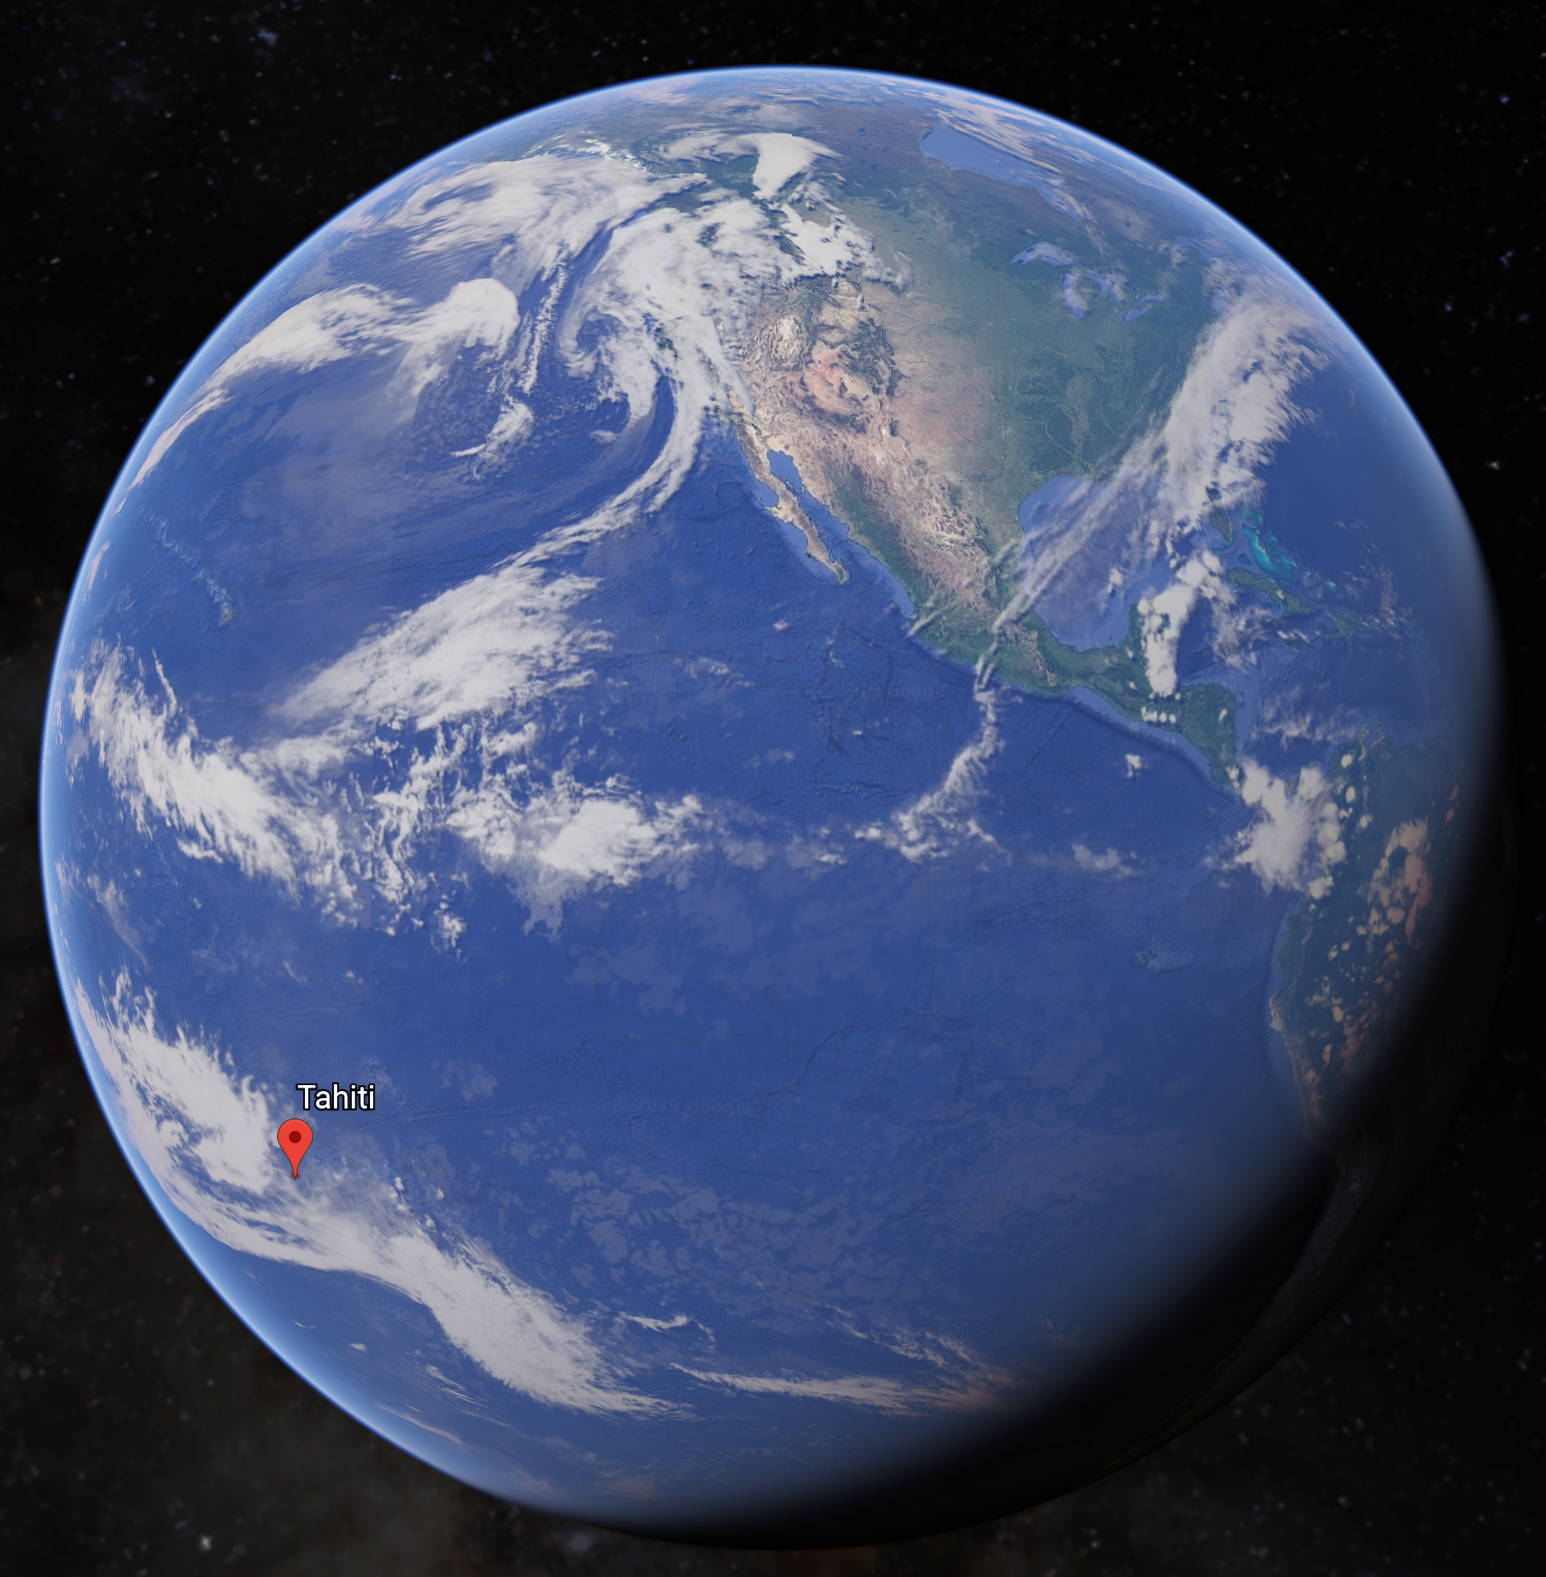
\includegraphics[height=5cm]{figures/tahitiloc.png}
		\label{tahitiloc}}
	\quad
	\subfloat[图片副标题]{
    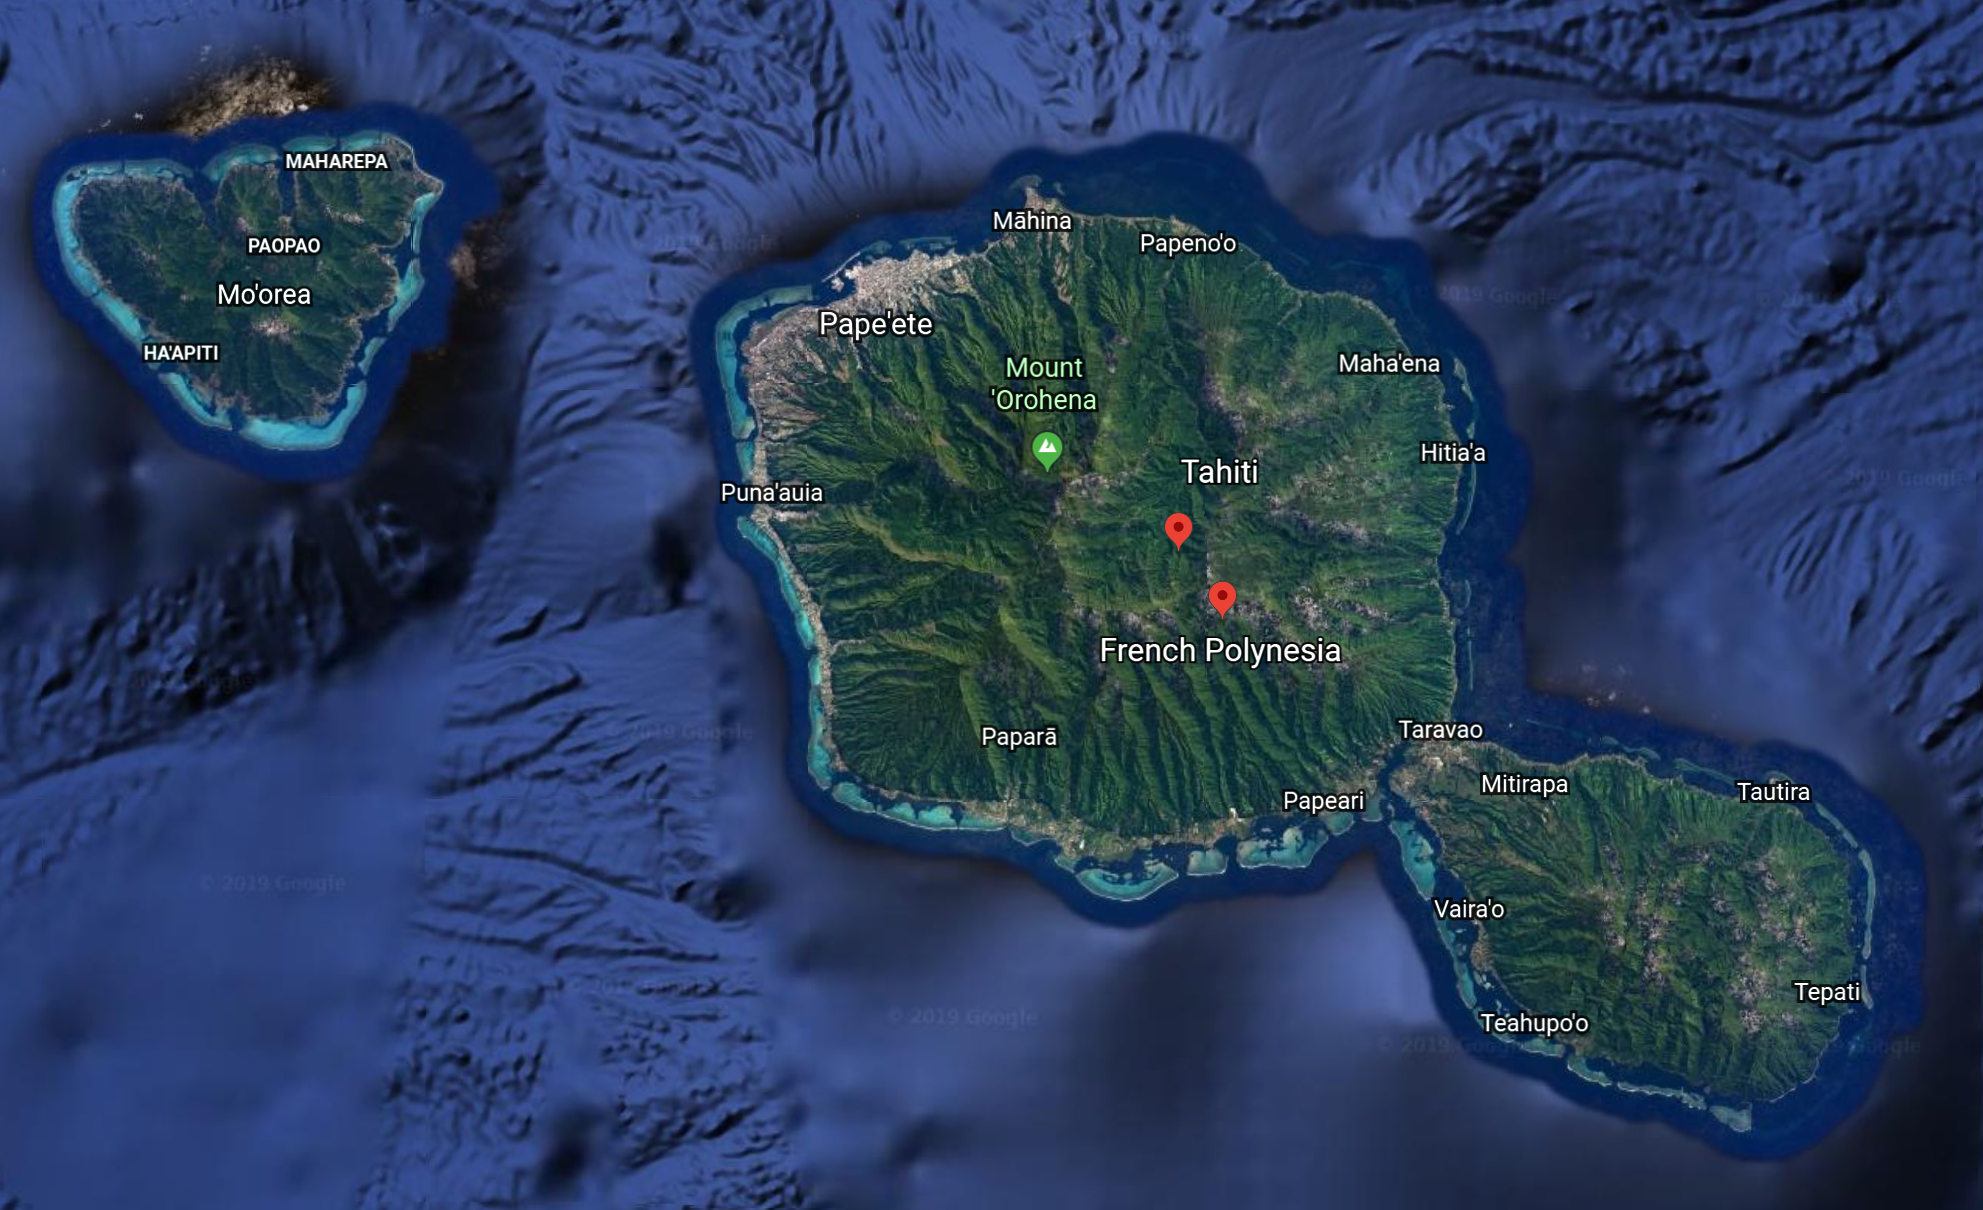
\includegraphics[height=5cm]{figures/tahitinear.png}
		\label{tahitinear}}
	\quad
	\caption{示例并排图片}
	\label{tahitilocation}
\end{figure}

\section{正文部分1}

此为一级标题。

\subsection{二级标题}

莫听穿林打叶声。何妨吟啸且徐行。竹杖芒鞋轻胜马。谁怕?一蓑烟雨任平生。料峭春风吹酒醒。微冷。山头斜照却相迎。回首向来萧瑟处。归去。也无风雨也无晴。\cite{tahitiworldatlas}.

\begin{figure}[!h]
  \centering
  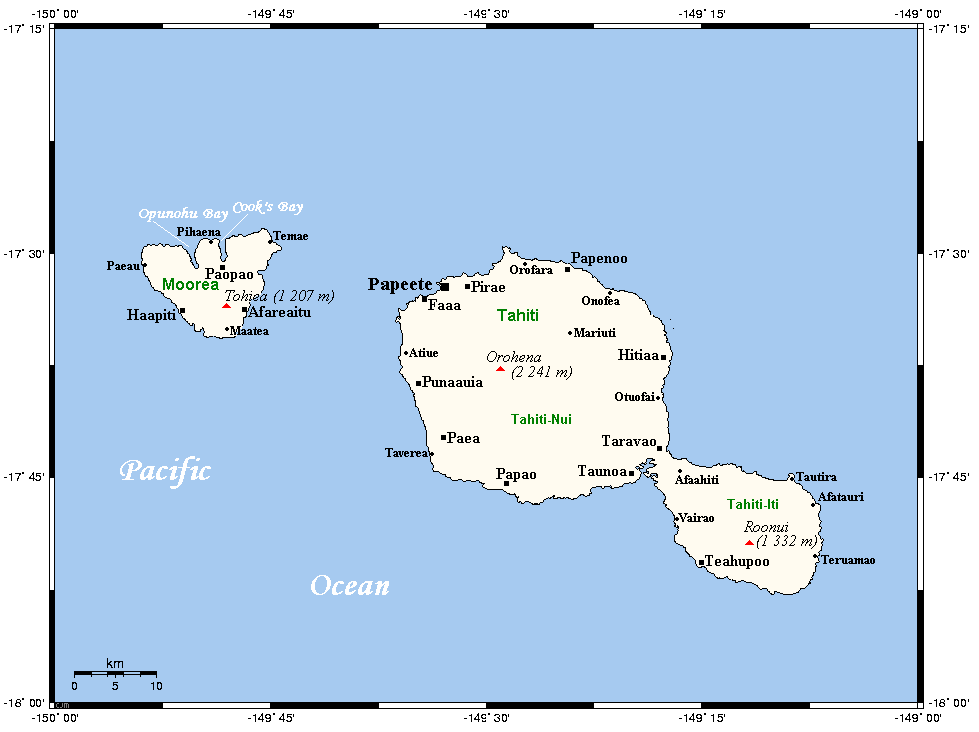
\includegraphics[height=6cm]{figures/TahitiMooreaMap.png}
  \caption{示例图片}
  \label{tmmap}
\end{figure}

\subsubsection{三级标题}

世事一场大梦,人生几度秋凉。夜来风叶已鸣廊,看取眉头鬓上。酒贱常愁客少,月明多被云妨。中秋谁与共孤光,把盏凄然北望。

\subsubsection{三级标题}

回首乱山横。不见居人只见城。谁似临平山上塔,亭亭。迎客西来送客行。归路晚风轻。一枕初寒梦不成。今夜残灯斜照处,荧荧。秋雨晴时泪不晴。

\section{正文部分2}

江汉西来,高楼下、蒲萄深碧。犹自带、岷峨雪浪,锦江春色。君是南山遗爱守,我为剑外思归客。对此间、风物岂无情,殷勤说。江表传,君休读。狂处士,真堪惜。空洲对鹦鹉,苇花萧瑟。独笑书生争底事,曹公黄祖俱飘忽。愿使君、还赋谪仙诗,追黄鹤。

\section{结论}

缥缈危楼紫翠间。良辰乐事古难全。感时怀旧独凄然。璧月琼枝空夜夜,菊花人貌自年年。不知来岁与谁看。

%% Switch back default alignment of IEEE Template section title
\patchcmd{\section}{\raggedright}{\centering}{}{}
\patchcmd{\section}{\normalsize}{\large\bfseries}{}{}

\appendices
\section{附录标题}
不适用请注释。

% % you can choose not to have a title for an appendix
% % if you want by leaving the argument blank
\section{第二个附录}
不适用请注释。


% % use section* for acknowledgment
\section*{致谢}

夜饮东坡醒复醉,归来仿佛三更。家童鼻息已雷鸣,敲门都不应,倚杖听江声。

长恨此身非我有,何时忘却营营。夜阑风静縠纹平。小舟从此逝,江海寄余生。

\ 

\raggedleft{——《临江仙·夜归临皋》}

\ifCLASSOPTIONcaptionsoff
  \newpage
\fi

%% Comment below line out if you want references in a new page.
%\newpage

%% Citation files store in ref.bib
\bibliographystyle{IEEEtran}
% argument is your BibTeX string definitions and bibliography database(s)
\bibliography{IEEEabrv,ref}


\end{document}


